% Options for packages loaded elsewhere
\PassOptionsToPackage{unicode}{hyperref}
\PassOptionsToPackage{hyphens}{url}
%
\documentclass[
]{article}
\usepackage{amsmath,amssymb}
\usepackage{iftex}
\ifPDFTeX
  \usepackage[T1]{fontenc}
  \usepackage[utf8]{inputenc}
  \usepackage{textcomp} % provide euro and other symbols
\else % if luatex or xetex
  \usepackage{unicode-math} % this also loads fontspec
  \defaultfontfeatures{Scale=MatchLowercase}
  \defaultfontfeatures[\rmfamily]{Ligatures=TeX,Scale=1}
\fi
\usepackage{lmodern}
\ifPDFTeX\else
  % xetex/luatex font selection
\fi
% Use upquote if available, for straight quotes in verbatim environments
\IfFileExists{upquote.sty}{\usepackage{upquote}}{}
\IfFileExists{microtype.sty}{% use microtype if available
  \usepackage[]{microtype}
  \UseMicrotypeSet[protrusion]{basicmath} % disable protrusion for tt fonts
}{}
\makeatletter
\@ifundefined{KOMAClassName}{% if non-KOMA class
  \IfFileExists{parskip.sty}{%
    \usepackage{parskip}
  }{% else
    \setlength{\parindent}{0pt}
    \setlength{\parskip}{6pt plus 2pt minus 1pt}}
}{% if KOMA class
  \KOMAoptions{parskip=half}}
\makeatother
\usepackage{xcolor}
\usepackage{longtable,booktabs,array}
\usepackage{calc} % for calculating minipage widths
% Correct order of tables after \paragraph or \subparagraph
\usepackage{etoolbox}
\makeatletter
\patchcmd\longtable{\par}{\if@noskipsec\mbox{}\fi\par}{}{}
\makeatother
% Allow footnotes in longtable head/foot
\IfFileExists{footnotehyper.sty}{\usepackage{footnotehyper}}{\usepackage{footnote}}
\makesavenoteenv{longtable}
\usepackage{graphicx}
\makeatletter
\newsavebox\pandoc@box
\newcommand*\pandocbounded[1]{% scales image to fit in text height/width
  \sbox\pandoc@box{#1}%
  \Gscale@div\@tempa{\textheight}{\dimexpr\ht\pandoc@box+\dp\pandoc@box\relax}%
  \Gscale@div\@tempb{\linewidth}{\wd\pandoc@box}%
  \ifdim\@tempb\p@<\@tempa\p@\let\@tempa\@tempb\fi% select the smaller of both
  \ifdim\@tempa\p@<\p@\scalebox{\@tempa}{\usebox\pandoc@box}%
  \else\usebox{\pandoc@box}%
  \fi%
}
% Set default figure placement to htbp
\def\fps@figure{htbp}
\makeatother
\setlength{\emergencystretch}{3em} % prevent overfull lines
\providecommand{\tightlist}{%
  \setlength{\itemsep}{0pt}\setlength{\parskip}{0pt}}
\setcounter{secnumdepth}{-\maxdimen} % remove section numbering
\usepackage{bookmark}
\IfFileExists{xurl.sty}{\usepackage{xurl}}{} % add URL line breaks if available
\urlstyle{same}
\hypersetup{
  hidelinks,
  pdfcreator={LaTeX via pandoc}}

\author{}
\date{}

\begin{document}

\section{Anatomie des Muscles : Guide pour le
Dessin}\label{anatomie-des-muscles-guide-pour-le-dessin}

\subsection{Table des Matières}\label{table-des-matiuxe8res}

\begin{enumerate}
\def\labelenumi{\arabic{enumi}.}
\tightlist
\item
  \hyperref[introduction]{Introduction}
\item
  \hyperref[muscles-du-haut-du-corps]{Muscles du Haut du Corps}

  \begin{itemize}
  \tightlist
  \item
    \hyperref[pectoraux]{Pectoraux}
  \item
    \hyperref[biceps]{Biceps}
  \item
    \hyperref[triceps]{Triceps}
  \item
    \hyperref[deltoides]{Deltoides}
  \item
    \hyperref[trapezes]{Trapezes}
  \end{itemize}
\item
  \hyperref[muscles-du-bas-du-corps]{Muscles du Bas du Corps}

  \begin{itemize}
  \tightlist
  \item
    \hyperref[abdominaux]{Abdominaux}
  \item
    \hyperref[quadriceps]{Quadriceps}
  \item
    \hyperref[ischio-jambiers]{Ischio-jambiers}
  \item
    \hyperref[mollets]{Mollets}
  \end{itemize}
\item
  \hyperref[muscles-du-dos]{Muscles du Dos}

  \begin{itemize}
  \tightlist
  \item
    \hyperref[grand-dorsal]{Grand Dorsal}
  \item
    \hyperref[rhomboides]{Rhomboides}
  \end{itemize}
\item
  \hyperref[conclusion]{Conclusion}
\item
  \hyperref[ressources-supplementaires]{Ressources Supplementaires}
\end{enumerate}

\begin{center}\rule{0.5\linewidth}{0.5pt}\end{center}

\subsection{Introduction}\label{introduction}

Dans l'art du dessin, maîtriser l'anatomie des muscles est crucial pour
rendre des personnages réalistes et expressifs. Ce guide va explorer les
muscles principaux du corps humain et leur rôle, avec des exemples
imagés pour illustrer leur position et leur fonction.

\begin{quote}
\textbf{Note :} Un bon dessinateur doit comprendre non seulement
l'emplacement des muscles, mais aussi comment ils réagissent lors du
mouvement.
\end{quote}

\begin{center}\rule{0.5\linewidth}{0.5pt}\end{center}

\subsection{Muscles du Haut du Corps}\label{muscles-du-haut-du-corps}

\subsubsection{Pectoraux}\label{pectoraux}

\begin{itemize}
\tightlist
\item
  \textbf{Nom complet} : \emph{Pectoralis Major}
\item
  \textbf{Fonction} : Adduction et rotation interne du bras.
\item
  \textbf{Emplacement} : Partie avant de la poitrine, reliant le sternum
  et l'humérus.
\end{itemize}

\begin{figure}
\centering
\pandocbounded{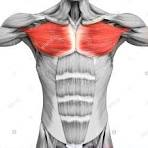
\includegraphics[keepaspectratio]{./images/pectoraux.jpg}}
\caption{Image des pectoraux}
\end{figure}

\begin{quote}
\textbf{Astuce pour le dessin} : Les pectoraux s'étirent et changent de
forme lorsque les bras sont élevés.
\end{quote}

\begin{center}\rule{0.5\linewidth}{0.5pt}\end{center}

\subsubsection{Biceps}\label{biceps}

\begin{longtable}[]{@{}
  >{\raggedright\arraybackslash}p{(\linewidth - 4\tabcolsep) * \real{0.3333}}
  >{\raggedright\arraybackslash}p{(\linewidth - 4\tabcolsep) * \real{0.3333}}
  >{\raggedright\arraybackslash}p{(\linewidth - 4\tabcolsep) * \real{0.3333}}@{}}
\toprule\noalign{}
\begin{minipage}[b]{\linewidth}\raggedright
Nom
\end{minipage} & \begin{minipage}[b]{\linewidth}\raggedright
Fonction
\end{minipage} & \begin{minipage}[b]{\linewidth}\raggedright
Emplacement
\end{minipage} \\
\midrule\noalign{}
\endhead
\bottomrule\noalign{}
\endlastfoot
\emph{Biceps Brachii} & Flexion du coude, rotation de l'avant-bras &
Partie avant supérieure du bras \\
\end{longtable}

\begin{figure}
\centering
\pandocbounded{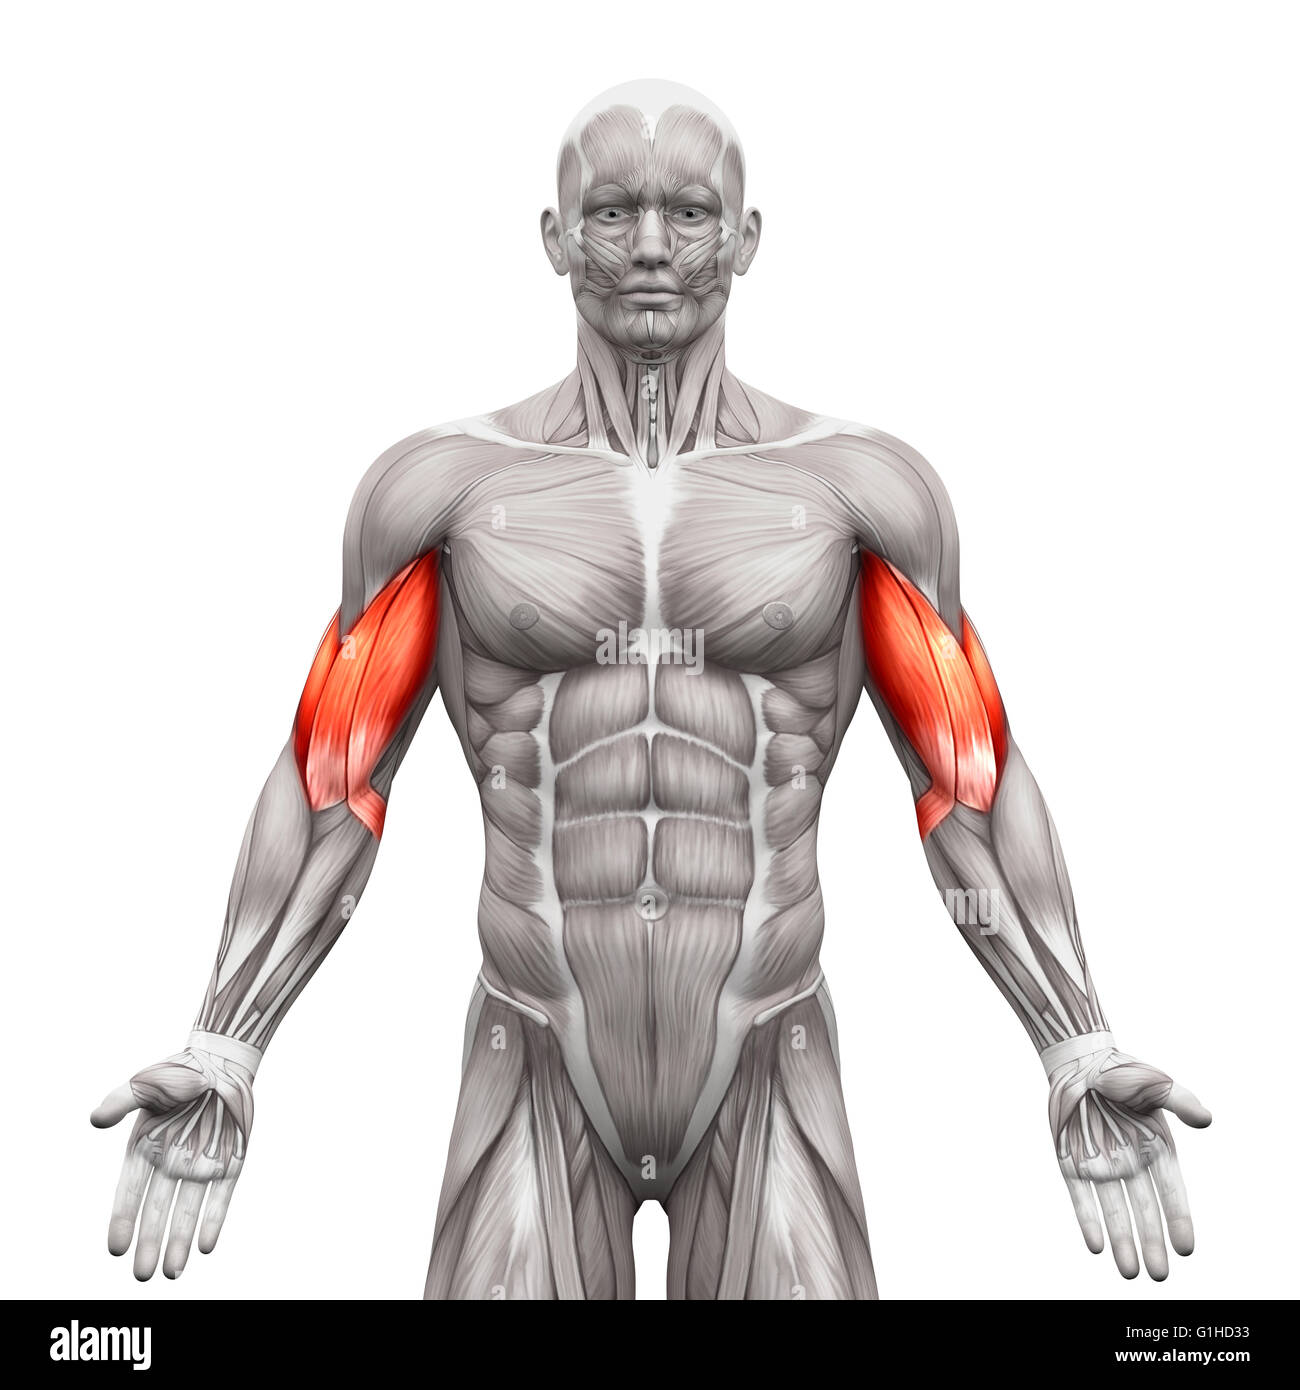
\includegraphics[keepaspectratio]{./images/biceps.jpg}}
\caption{Image des biceps}
\end{figure}

\begin{center}\rule{0.5\linewidth}{0.5pt}\end{center}

\subsubsection{Triceps}\label{triceps}

Les \textbf{triceps brachiaux} sont des muscles à trois chefs situés à
l'arrière du bras. Leur principale fonction est l'extension du coude.

\begin{itemize}
\tightlist
\item
  \textbf{Chefs} :

  \begin{itemize}
  \tightlist
  \item
    \emph{Long chef}
  \item
    \emph{Chef latéral}
  \item
    \emph{Chef médial}
  \end{itemize}

  \begin{figure}
  \centering
  \pandocbounded{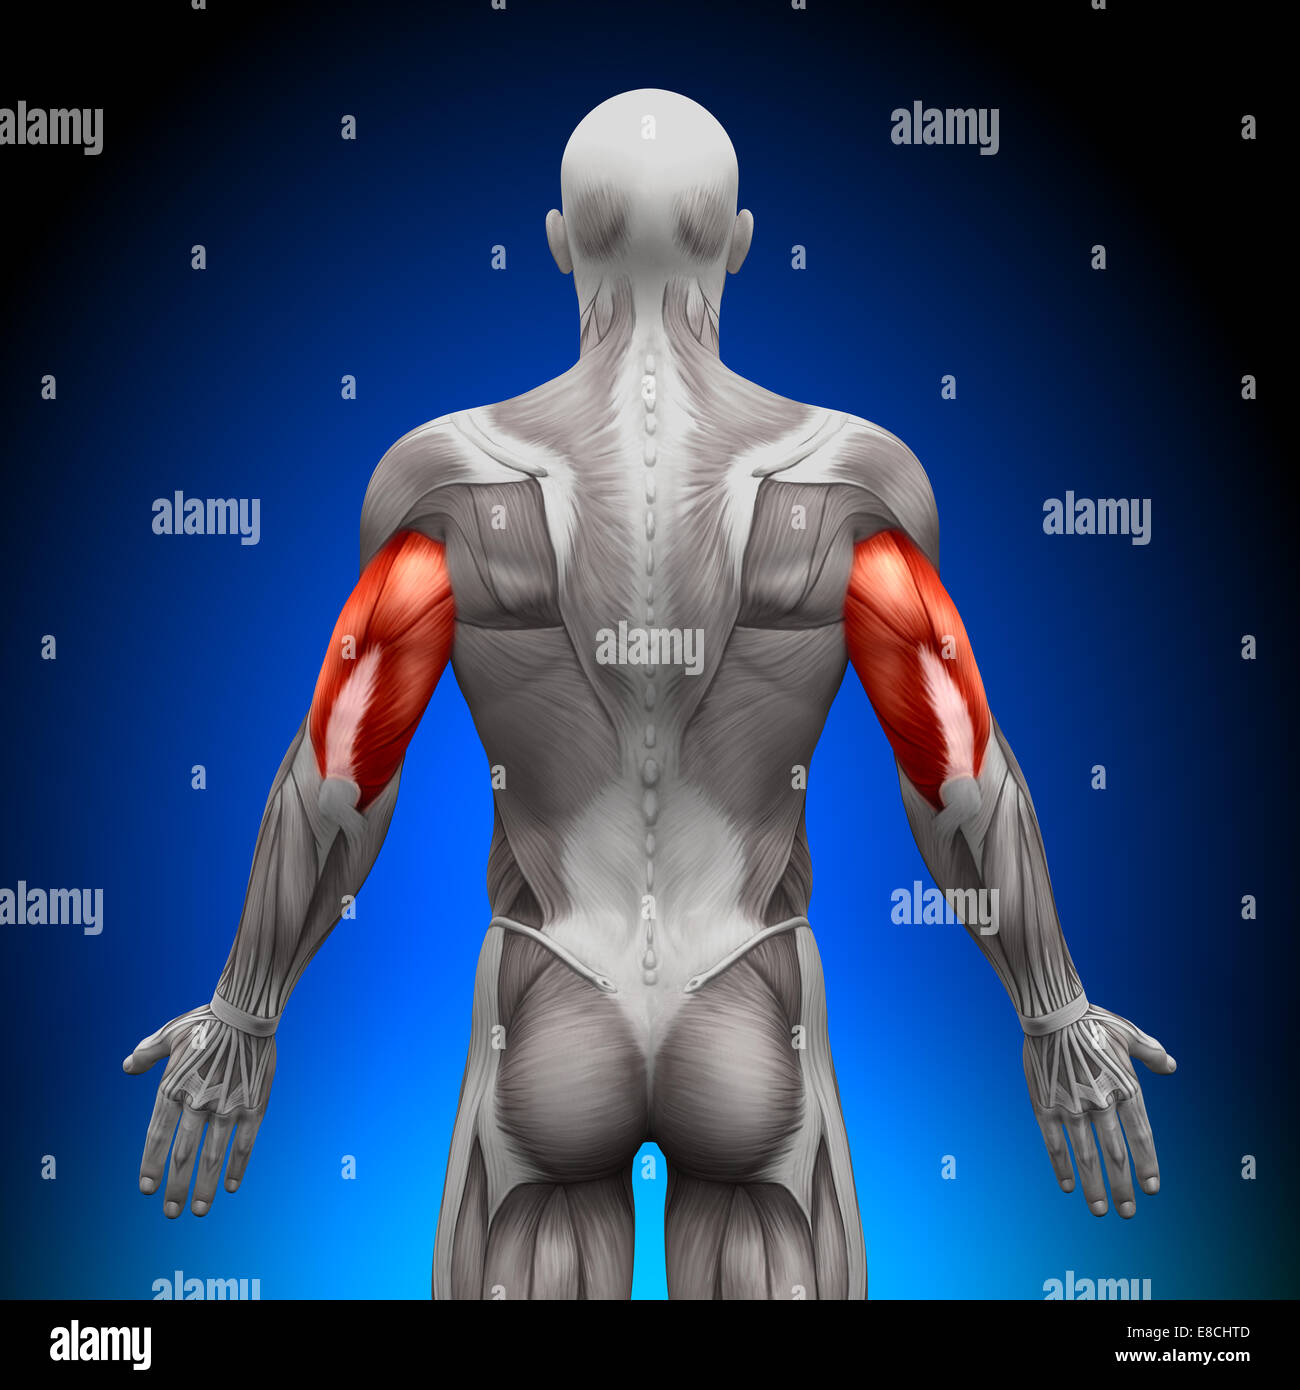
\includegraphics[keepaspectratio]{./images/triceps.jpg}}
  \caption{Image des triceps}
  \end{figure}
\end{itemize}

\begin{quote}
\textbf{À retenir} : Les triceps sont essentiels pour montrer la
puissance lors des poses où les bras sont tendus.
\end{quote}

\begin{center}\rule{0.5\linewidth}{0.5pt}\end{center}

\subsubsection{Deltoides}\label{deltoides}

Les deltoïdes sont les muscles arrondis de l'épaule, répartis en trois
faisceaux. Ils permettent différents mouvements de l'épaule.

\begin{enumerate}
\def\labelenumi{\arabic{enumi}.}
\tightlist
\item
  \textbf{Faisceau antérieur} (avant) : Levée du bras vers l'avant.
\item
  \textbf{Faisceau latéral} (milieu) : Abduction du bras.
\item
  \textbf{Faisceau postérieur} (arrière) : Extension du bras vers
  l'arrière.
\end{enumerate}

\begin{figure}
\centering
\pandocbounded{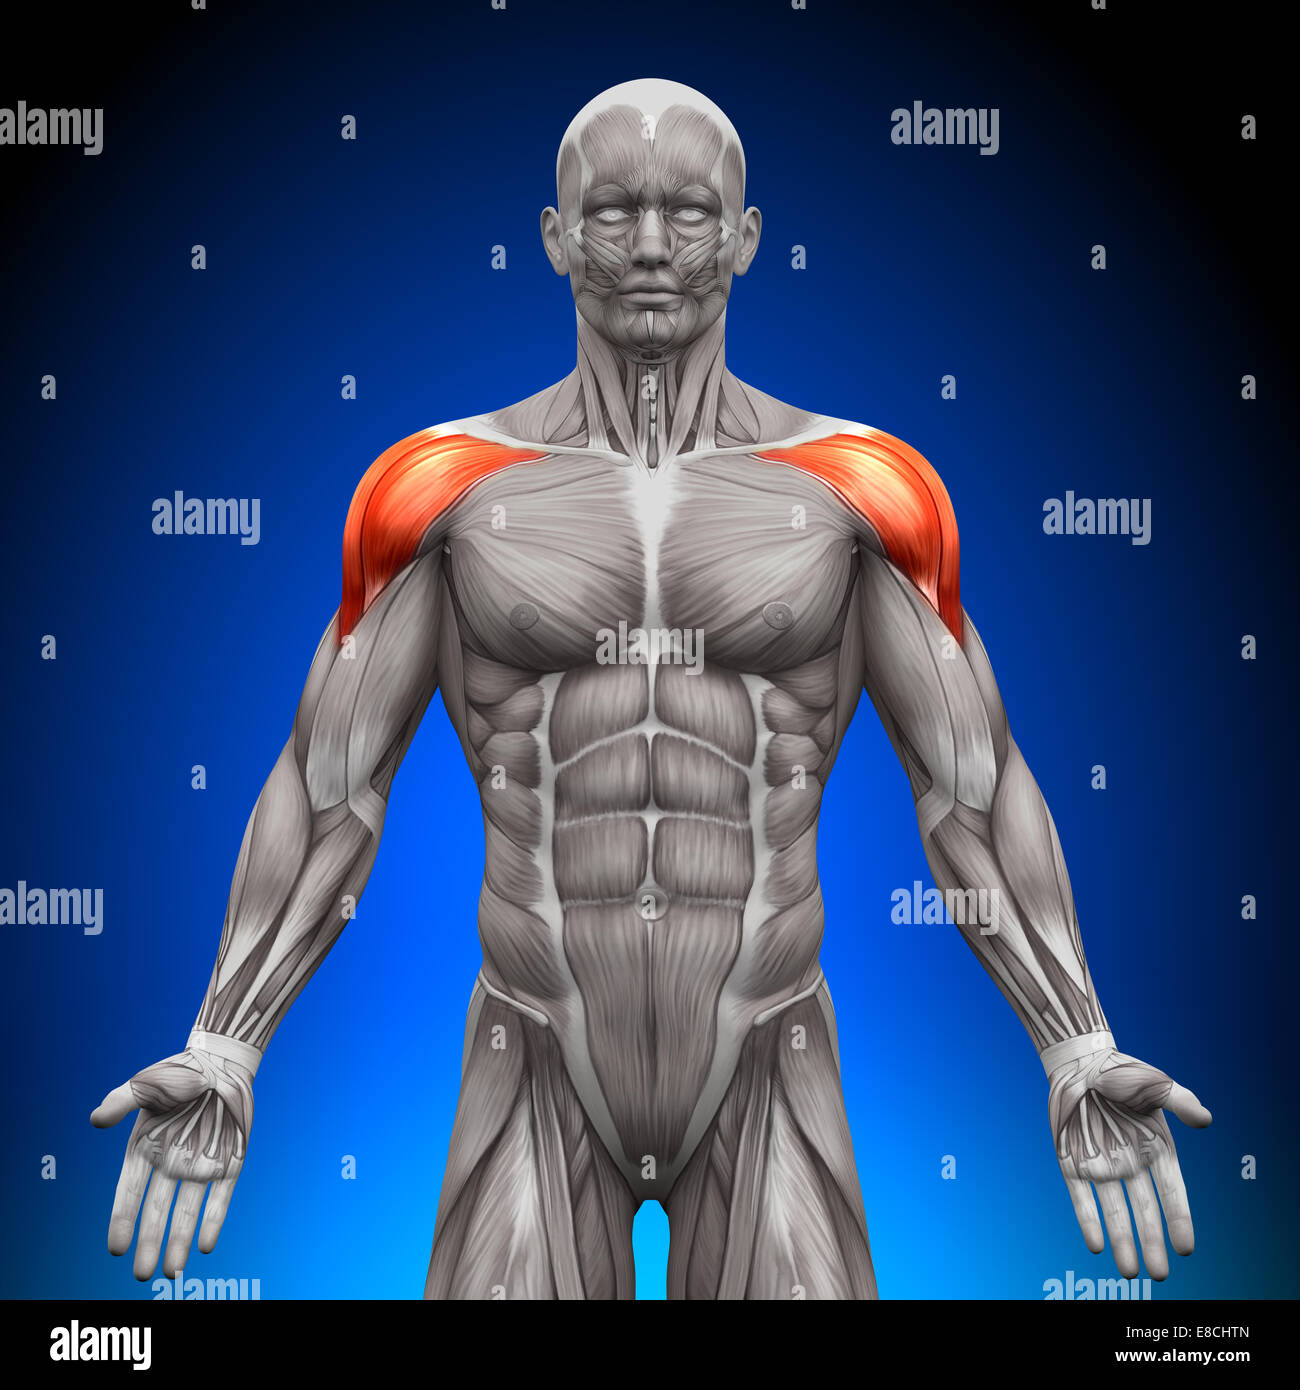
\includegraphics[keepaspectratio]{./images/deltoides.jpg}}
\caption{Image des deltoïdes}
\end{figure}

\begin{center}\rule{0.5\linewidth}{0.5pt}\end{center}

\subsubsection{Trapezes}\label{trapezes}

Le \textbf{trapèze} est un large muscle en forme de losange s'étendant
de la nuque au milieu du dos.

\begin{itemize}
\tightlist
\item
  \textbf{Fonction} : Stabilisation des omoplates et mouvements de la
  tête et du cou.
\item
  \textbf{Emplacement} : Partie supérieure du dos.
\end{itemize}

\begin{longtable}[]{@{}ll@{}}
\toprule\noalign{}
Fonction principale & Mouvement associé \\
\midrule\noalign{}
\endhead
\bottomrule\noalign{}
\endlastfoot
Élever les omoplates & Haussement d'épaules \\
Abaisser les omoplates & Mouvements descendants des bras \\
\end{longtable}

\begin{figure}
\centering
\pandocbounded{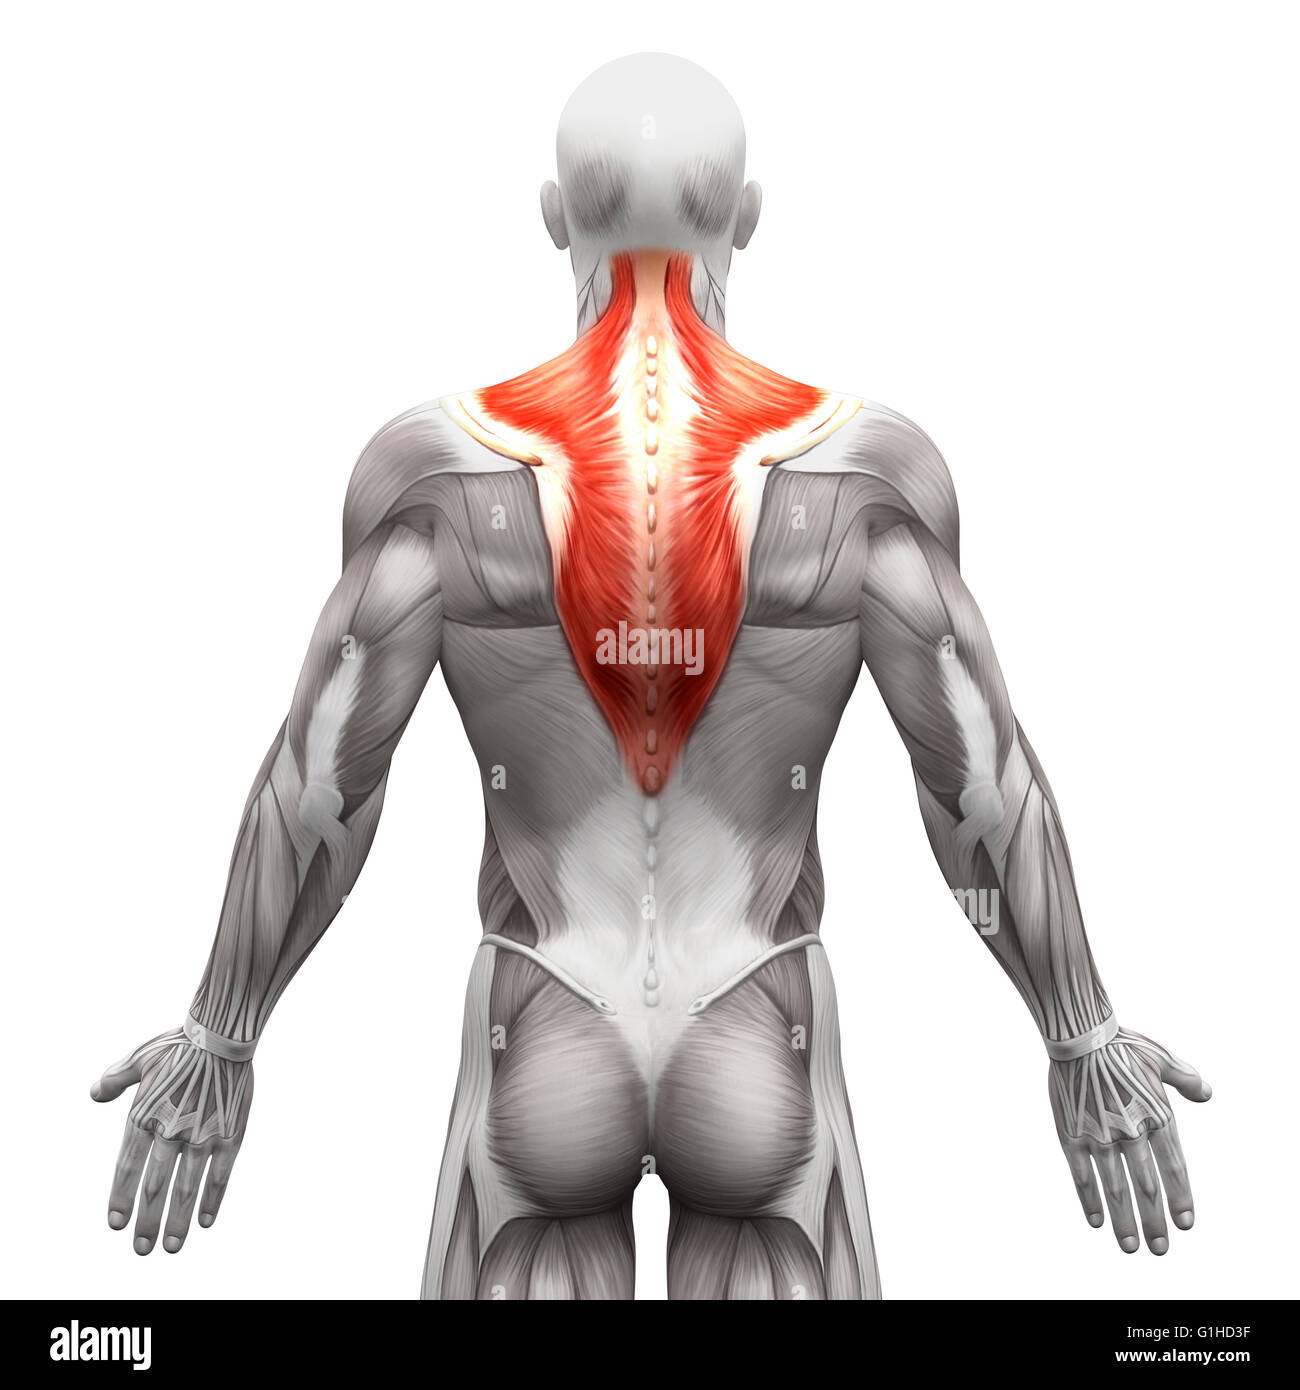
\includegraphics[keepaspectratio]{./images/trapezes.jpg}}
\caption{Image des trapèzes}
\end{figure}

\begin{center}\rule{0.5\linewidth}{0.5pt}\end{center}

\subsection{Muscles du Bas du Corps}\label{muscles-du-bas-du-corps}

\subsubsection{Abdominaux}\label{abdominaux}

Les abdominaux, en particulier le \textbf{grand droit de l'abdomen},
sont un groupe de muscles situés à l'avant du torse. Ils jouent un rôle
important dans la flexion de la colonne vertébrale et la stabilisation
du tronc.

\begin{itemize}
\tightlist
\item
  \textbf{Parties principales} :

  \begin{itemize}
  \tightlist
  \item
    \emph{Grand droit} : Les fameuses ``tablettes de chocolat''.
  \item
    \emph{Obliques} : Muscles latéraux responsables de la rotation du
    tronc.
  \end{itemize}
\end{itemize}

\begin{center}\rule{0.5\linewidth}{0.5pt}\end{center}

\subsubsection{Quadriceps}\label{quadriceps}

Les \textbf{quadriceps} sont un groupe de quatre muscles situés à
l'avant de la cuisse. Ils permettent l'extension du genou.

\begin{itemize}
\tightlist
\item
  \textbf{Muscles du quadriceps} :

  \begin{enumerate}
  \def\labelenumi{\arabic{enumi}.}
  \tightlist
  \item
    \emph{Droit fémoral}
  \item
    \emph{Vaste latéral}
  \item
    \emph{Vaste intermédiaire}
  \item
    \emph{Vaste médial}
  \end{enumerate}
\end{itemize}

\begin{figure}
\centering
\pandocbounded{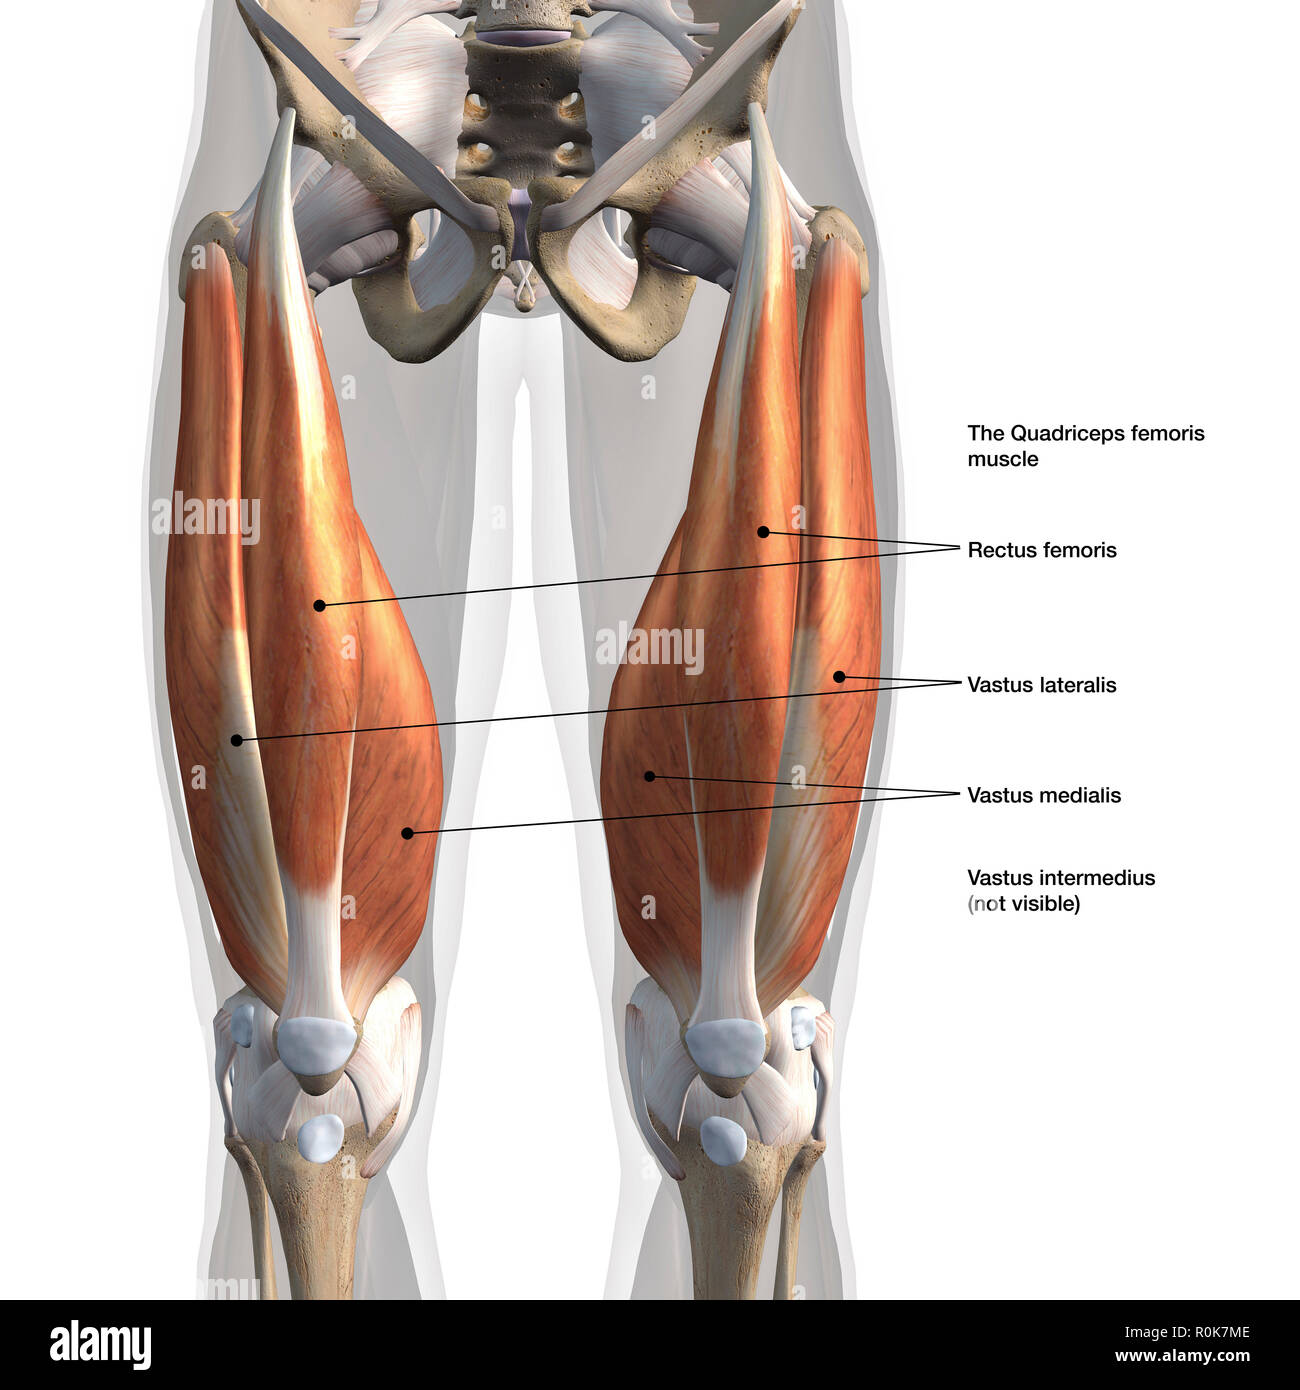
\includegraphics[keepaspectratio]{./images/quadriceps.jpg}}
\caption{Image des quadriceps}
\end{figure}

\begin{center}\rule{0.5\linewidth}{0.5pt}\end{center}

\subsubsection{Ischio-jambiers}\label{ischio-jambiers}

Les \textbf{ischio-jambiers} se trouvent à l'arrière de la cuisse et
sont responsables de la flexion du genou.

\begin{itemize}
\tightlist
\item
  \textbf{Fonction} : Permet de plier la jambe à partir du genou.
\item
  \textbf{Emplacement} : De l'os de la hanche à l'arrière du genou.
\end{itemize}

\begin{figure}
\centering
\pandocbounded{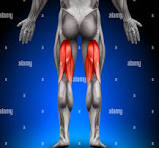
\includegraphics[keepaspectratio]{./images/ischio-jambiers.jpg}}
\caption{Image des ischio-jambiers}
\end{figure}

\begin{center}\rule{0.5\linewidth}{0.5pt}\end{center}

\subsubsection{Mollets}\label{mollets}

Les \textbf{mollets} sont composés de deux principaux muscles :

\begin{itemize}
\tightlist
\item
  \textbf{Gastrocnémien} : Permet la flexion plantaire du pied.
\item
  \textbf{Soléaire} : Soutient le gastrocnémien lors de la marche.
\end{itemize}

\begin{figure}
\centering
\pandocbounded{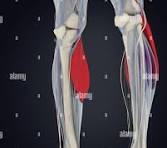
\includegraphics[keepaspectratio]{./images/mollets.jpg}}
\caption{Image des mollets}
\end{figure}

\begin{center}\rule{0.5\linewidth}{0.5pt}\end{center}

\subsection{Muscles du Dos}\label{muscles-du-dos}

\subsubsection{Grand Dorsal}\label{grand-dorsal}

Le \textbf{grand dorsal} est un muscle large et plat qui recouvre la
partie inférieure du dos. Il est principalement responsable des
mouvements de tirage vers l'arrière.

\begin{itemize}
\tightlist
\item
  \textbf{Fonction} : Adduction, extension et rotation interne du bras.
\item
  \textbf{Emplacement} : Partie inférieure et latérale du dos.
\end{itemize}

\begin{figure}
\centering
\pandocbounded{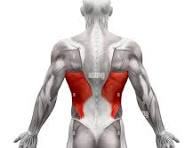
\includegraphics[keepaspectratio]{./images/grand_dorsal.jpg}}
\caption{Image du grand dorsal}
\end{figure}

\begin{center}\rule{0.5\linewidth}{0.5pt}\end{center}

\subsubsection{Rhomboides}\label{rhomboides}

Les \textbf{rhomboïdes} sont situés entre les omoplates et la colonne
vertébrale.

\begin{itemize}
\tightlist
\item
  \textbf{Fonction} : Rétraction et stabilisation des omoplates.
\item
  \textbf{Emplacement} : Entre la colonne thoracique et les omoplates.
\end{itemize}

\begin{figure}
\centering
\pandocbounded{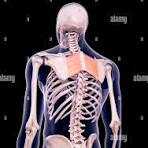
\includegraphics[keepaspectratio]{./images/rhomboides.jpg}}
\caption{Image des rhomboïdes}
\end{figure}

\begin{center}\rule{0.5\linewidth}{0.5pt}\end{center}

\subsection{Conclusion}\label{conclusion}

L'anatomie des muscles est essentielle pour le dessin réaliste du corps
humain. Comprendre comment les muscles se contractent, se détendent et
influencent la forme du corps permet de mieux représenter les poses et
les mouvements.

\begin{quote}
\textbf{Citation à retenir :} ``Un bon dessin est une fusion de
connaissance anatomique et d'observation attentive.'' -- \emph{Léonard
de Vinci}
\end{quote}

\begin{center}\rule{0.5\linewidth}{0.5pt}\end{center}

\subsection{Ressources
Supplementaires}\label{ressources-supplementaires}

\begin{itemize}
\tightlist
\item
  \href{https://www.proko.com/}{Anatomie pour Artistes - Proko}
\item
  Human Anatomy for Artists - Eliot Goldfinger
\item
  \href{https://www.pinterest.com/}{Drawings of Anatomy on Pinterest}
\item
  \href{https://www.alamy./images.fr/}{Alamy ./images}
\end{itemize}

\end{document}
